\section{DRAM Device Architecture}\label{sec:dram-arch} In a DRAM IC, arrays of
bit cells are hierarchically arranged into multiple parallel \emph{banks}.
Banks provide the primitive level of concurrency in a DRAM memory system. They
can service independent requests, assuming they do not simultaneously require
shared resources like the data, address and command buses.  Multiple DRAM ICs
can be arranged in parallel to widen the data bus; address and command buses
fan out to each IC. For more concurrency, and to support larger memory
capacities, multiple \emph{ranks} of DRAM devices may be used. Here, generally,
the command and data buses are shared between all ranks, with a one-hot
chip-select indicating which rank a command is addressed to.

A basic DRAM operation requires a series of three commands: \emph{activate
(ACT)}, \emph{column access~(CAS)}, and \emph{precharge~(PRE)}. Initially, the
bitlines of the DRAM-cell array are precharged to VDD/2, and DRAM-cells are
isolated from the bitline by a single access transistor. First, a row must be
\emph{opened}. The ACT command achieves this by enabling a word-line of the
array corresponding to a single \emph{row} of the bank. Charge sharing between
the cells of the now-open row and the bitlines of the array create
perturbations in the bitline voltages that are sensed by the array of
differential sense-amps.  This is temporarily destructive: the bit-cell voltage
is driven to approximately VDD/2. However, after the initial ``sense" phase,
the amps drive the bitline voltage back towards VCC or GND based on the
state of the bit cell, restoring the cell voltage. The
sense-amps also act as a \emph{row buffer}, storing the sensed state of
the row indefinitely.

A CAS command then selects a subset of the row buffer to read or write~(CASR
and CASW commands respectively). In double-data rate~(DDR) DRAM, data is
bursted over successive rising and falling clock edges.  While the row buffer
remains open, the row can be accessed by issuing new CAS commands. 

Finally, to access a row not stored in the buffer, a PRE command must be issued
to \emph{close} the row, disabling the wordline, and precharging bitline back to
VDD/2 to prepare for a new access.

\begin{figure}
	\centering
	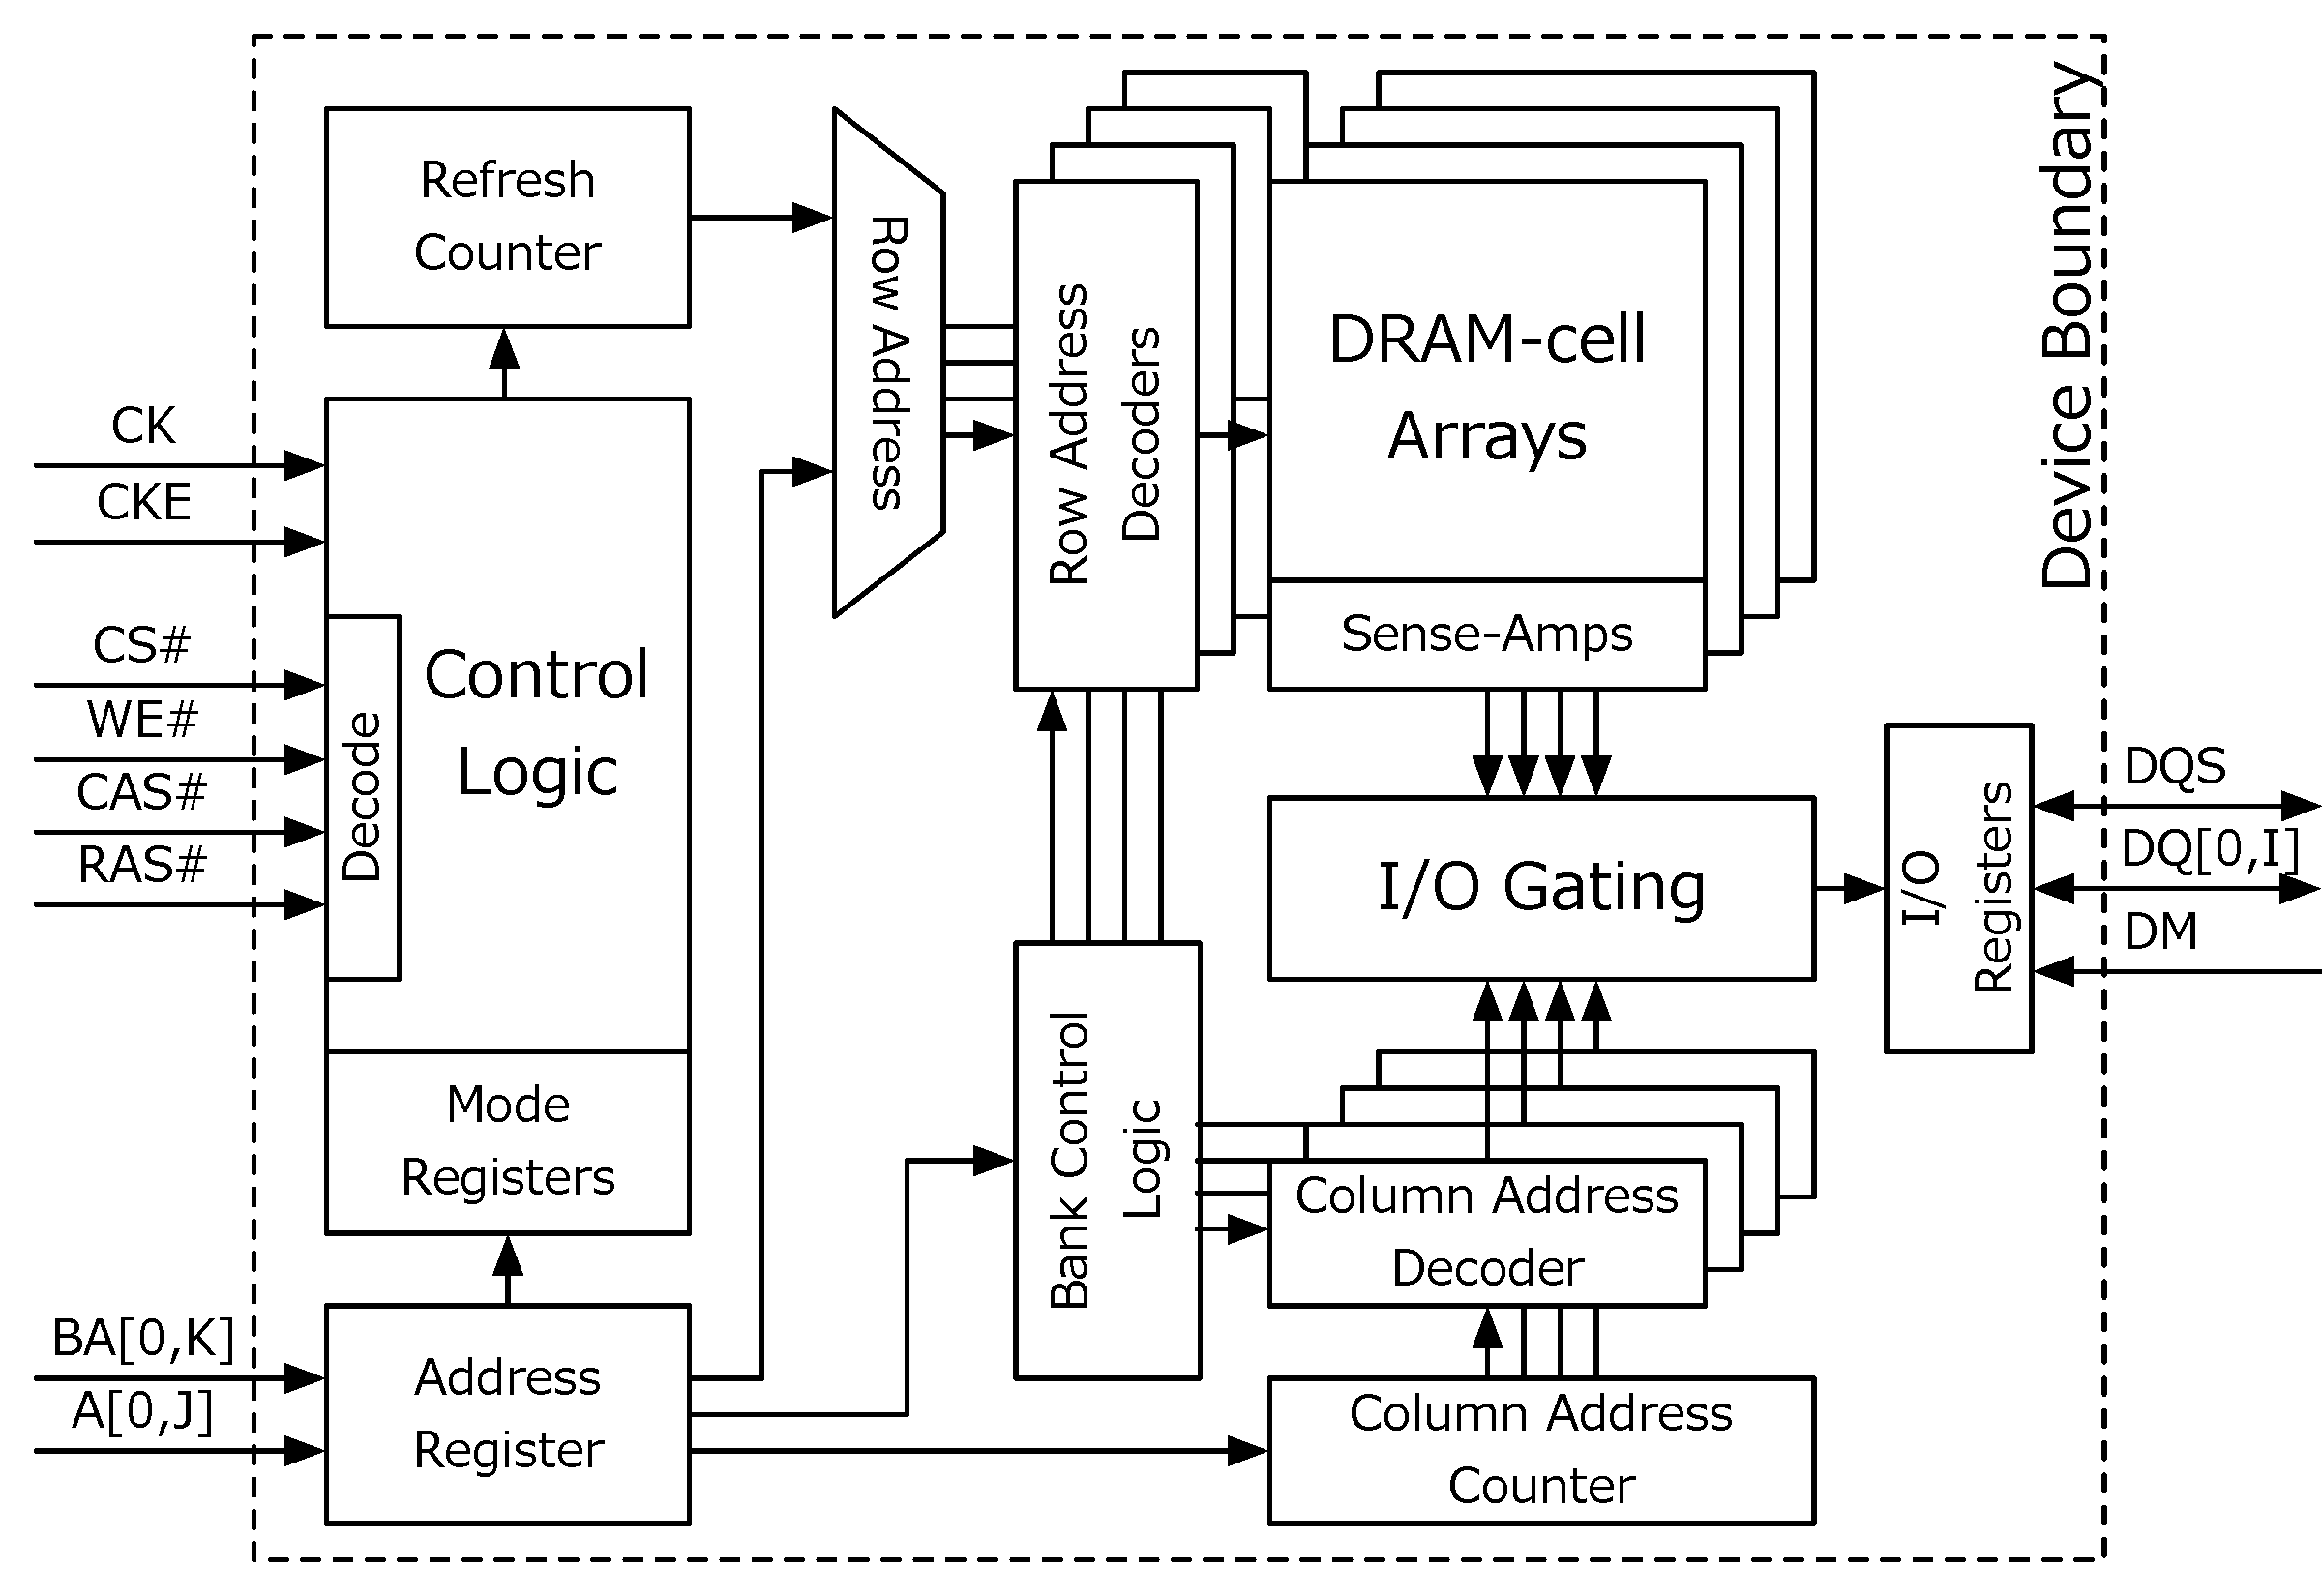
\includegraphics[width=16cm]{figures/dram-device.pdf}
    \caption{A simplified diagram of the organization of a typical DRAM device.}
	\label{fig:dram-device}
\end{figure}

DRAM is named dynamic RAM because it gradually loses its stored state over time
as bit-cell capacitors leak. DRAM-cell retention rates vary both on a single
die and between dies and are highly sensitive to temperature~(warmer cells leak
faster). To maintain their state, DRAM cells must be periodically ``refreshed".
Activating a row of cells is sufficient to refresh them. As part of the DRAM
standards, JEDEC mandates cells must be refreshed on-average once every 64 ms;
an interval they have maintained from DDR through DDR4. Since activations to
every row cannot generally be guaranteed, DRAM devices are refreshed explicitly
with a refresh command~(REF). To reduce complexity, this command refreshes a
constant number of contiguous rows beginning at a base row address in all banks
concurrently.  The base address is incremented which each REF command. DRAM
manufacturers generally have kept the number of refresh commands required to
iterate through the entire array constant: 8192 commands per 64 ms interval, or
one on average every 7.8 $\mu s$.  Hence, refresh commands take longer to
execute on devices with more rows per bank.

A complete list of timings required to model a generic DDR protocol is give in
table \ref{tbl:dram-timings}. These have been taken, with some modification,
from \textit{Memory Systems: Cache, DRAM, Disk}\cite{drambook}.

\begin{table}[htb]
\begin{center}
\resizebox{\textwidth}{!}{%
    \begin{tabular}{|p{0.20\textwidth}|p{0.8\textwidth}|}
    \hline
    \textbf{Name} & \textbf{Description} \\
    \hline
    \hline
    \textbf{$t_{AL}$} & Additive Latency. Additional latency added to column access commands. \\
    \textbf{$t_{CAS}$~($t_{CL}$)} & Column Access Strobe latency. Delay between
    when a CASR command is received and when the first beat of read data is
    returned. \\ \textbf{$t_{CCD}$} & Column-to-Column Delay. Minimum duration
    between two consecutive column commands. \\ \textbf{$t_{CMD}$} & Command
    transport duration. The duration a command occupies the command bus. \\
    \textbf{$t_{CWD}$~($t_{WL}$)} & Column Write Delay. The delay between a
    CASW command and the when the controller must present the first beat of
    write data. \\
    \textbf{$t_{FAW}$} & Four row Activation Delay. A rolling time window
    during which only four row activations may be made to all banks of a DRAM
    device. \\
    \textbf{$t_{RAS}$} & Row Access Strobe. The minimum duration after an ACT
    command that the row must be kept open before issuing a precharge command
    to close it. \\
    \textbf{$t_{RC}$} & Row Cycle time. The minimum duration required
    to open, and close a row. $t_{RC} = t_{RAS} + t_{RP}$ \\
    \textbf{$t_{REFI}$} & Refresh Interval. The average period of time between refresh commands. \\
    \textbf{$t_{RCD}$} & Row-to-Column Delay. The minimum duration after
    activation column commands may be issued to the newly-opened row.  \\
    \textbf{$t_{RFC}$} & ReFresh Cycle time. The minimum duration after a refresh
    command that activation commands may be issued. \\
    \textbf{$t_{RP}$} & Row Precharge delay. The minimum duration after a
    precharge command that an ACT to the same bank may be issued. \\
    \textbf{$t_{RRD}$} & Row-to-Row Delay. The minimum duration between ACT commands to the same bank. \\
    \textbf{$t_{RTP}$} & Read-To-Precharge delay. The mimimum duration after a CASR command that a precharge may be issued to the same row. \\
    \textbf{$t_{RTRS}$} & Rank-To-Rank Switching delay. Accounts for time to change termination schemes on DQ and DQS buses when switching between ranks. \\
    \textbf{$t_{WR}$} & Write Recovery time. The minimum duration after a CASW command that a precharge command may be issued to the same row. \\
    \textbf{$t_{WTR}$} & Write TurnaRound Time. The minimum duration after a CASW command that a CASR may be issued to the same row. \\
    \hline
\end{tabular}}
\end{center}
\caption{A list of key timings for a conventional DDRx SDRAM}
\label{tbl:dram-timings}
\end{table}%

\clearpage
\section{DRAM Controller Architecture}

A DRAM controller is responsible for responding to memory
requests from one or more requestors by scheduling those requests over its
attached memories as a judicious stream of DRAM commands.

Memory access scheduling~(MAS) is the process by which, for a given cycle, a
controller selects a single DRAM command to be issued from a legal set. Legal
commands are constrained by the current state of each bank, the availability
of shared resources like the command and data buses, and timing constraints
imposed by the DRAM standard. Good MAS policies strike a delicate balance
between minimizing latency, maintaining quality-of-service guarantees across
multiple threads of execution, maximizing bandwidth, and minimizing power.
There are plethora of academic papers on MAS policies, and still more
industrial patents on the subject. In this work we consider two popular MAS policies. 

\subsection{First-Come First-Serve~(FCFS) Policy}\label{sec:fcfs} Commands for the
oldest pending memory reference are issued first. This is the simplest MAS
policy, but tends to under-utilize available DRAM bandwidth as younger requests
that may hit in the row-buffer are not issued before older commands that miss.
FCFS schedulers are common in older machines, and those that present few
concurrent memory requests.

\subsection{First-Ready FCFS~(FR-FCFS)~\cite{frfcfs} Policy}\label{sec:frfcfs}
First, ready~(legally issuable) column commands are prioritized over ready row
commands. Second, commands for older references are prioritized over younger
ones. This permits younger but ready column commands to be issued before older
row commands. FR-FCFS is a relatively simple scheme that improves bandwidth
utilization considerably. It is the de facto standard against which new MAS
policies for machines with a single stream of memory references~(like
single-core out-of-order machines), are compared.

\section{Power Consumption in DRAM Memories}\label{sec:dram-power}

We can divided DRAM power consumption into six different classes: activation
(including precharge), read, write, termination, refresh, and background power.

Activation is generally the largest contributor to DRAM power consumption.  In an
effort to maximize areal density and reduce cost-per-bit, DRAM sub-arrays have
very long, high capacitance bit lines, which are driven to VDD or ground during
the restore phase of an activation. Moreover, DRAM rows are long, with
thousands of bitlines are simultaenously charged or discharged in a single
activation, leading to large peak-current draw. In order to stay within a power
envelope where DRAM ICs can be cooled passively without heatsinks, DRAM
manufacturers introduced the $t_{RRD}$ and $t_{FAW}$ constraints described in
table\ref{tbl:dram-timings} in DDR3.

Read and write power consumption accounts accounts for the power dissipated as
read or write data is driven to and from the I/Os of the chip to the various
sub-arrays, as well as the power used to decode the read or write command.
Shorter bursts consume less power.

Refresh power accounts for the power lost during the successive activations and
precharges of a refresh command. It is a growing contributor as modern DRAM ICs
trend towards higher row counts and thus must refresh more rows per refresh
command, forcing the IC to spend longer in refresh (higher $t_{RFC}$).

Termination power accounts for the power dissipated in termination resistors
during a write, and by the output buffers of a DRAM IC during a read. In
multi-rank systems, this includes power is also dissipated in the termination
resistors of ranks not being addressed.

Finally, background power accounts for leakage of various circuits within the
IC. Here there are two dimensions of note. Firstly, activated banks
leak more than precharged banks. Second, powered-down banks~(CKE low) leak less
than powered-up banks~(CKE high).


\section{Simulation of DRAM-based Memory Systems}

The current state of the art in DRAM simulation in academia are cycle-accurate
software simulators like DRAMSim2~\cite{dramsim}, Ramulator~\cite{ramulator} and
USIMM~\cite{usimm}. These models generate DRAM command streams that have been
validated against industrial models~(for some standards). Both Ramulator and
DRAMSim2 can be easily integrated into Gem5~\cite{gem5}, though gem5 includes a
detailed event-based model of its own~\cite{gem5event}. In trace-driven mode,
operating at full throughput and only as a timing-model, these cycle-accurate
models simulate at frequencies ranging from hundreds of KHz to ones of
MHz~\cite{ramulator}.

In order to model power, Micron has described a strategy that assigns an
average current draw to each of the six states described in
section~\ref{sec:dram-power}. These currents can be found in Micron data
sheets, and must be derated according to supply voltage and frequency.
DRAMSim2 directly implements this strategy, integrating the approriate current
based on the state of the simulated memories. Micron provides spreadsheets that
approximately implement this strategy for a variety of popular DRAM
technologies. Thus, with measurements of the relative activities, one can
generate estimate DRAM power dissipation as post-processing step.  These
approaches can also be used in an FPGA simulation, as sufficiently detailed
FPGA models can add instrumentation for the necessary events.

One limitation of the Micron approach, is that it does not account for the
power dissipation of the controller itself. However, for modest memory
controller implementations, this should be small.
